\documentclass[a4paper,12pt,twoside,openany,notitlepage]{book}
\usepackage{amssymb}
\usepackage[utf8]{inputenc}
\usepackage{polski}
\usepackage[OT4]{fontenc}
\usepackage{amsmath}
\usepackage{amsfonts}
\usepackage[T1]{fontenc}
\usepackage{graphicx}
\graphicspath{ {images/} }
\usepackage{tabu}
\usepackage{pgfplots}
\usepackage[nottoc]{tocbibind}
\usepackage{fancyhdr}

\pagestyle{fancy}
\fancyhf{}
\fancyhead[LE,RO]{\leftmark}
\fancyhead[RE,LO]{\thepage}

\begin{document}

% ustawia odpowiednie marginesy
\newpage
\thispagestyle{empty}
\mbox{}

\newpage
\thispagestyle{empty}
\mbox{}
    \begin{center}
        \vspace*{1cm}
        
        \large
        \textbf{WYDZIAŁ INFORMATYKI, ELEKTRONIKI I TELEKOMUNIKACJI}
        
        \vspace{0.8cm}
        KATEDRA TELEKOMUNIKACJI

        \vspace{4cm}
        \Large
        \textbf{PRACA DYPLOMOWA INŻYNIERSKA}

        \vspace{0.8cm}
        \large
        \textit{Wdrożenie systemu wczesnego wykrywania ataków typu DDoS w środowisku
        sieci sterowanych programowo SDN}

        \vspace{0.5cm}
        \small
        \textit{Implementation of selected early DDoS detection system in
          Software Defined Networks}

      \end{center}

        \vfill
        
        \noindent
        Autor: \textit{Kacper Mentel}\\
        Kierunek studiów: \textit{Teleinformatyka}\\
        Opiekun pracy: \textit{dr inż. Artur Lasoń}\\

      \begin{center}
        Kraków, 2017
      \end{center}

\newpage
\thispagestyle{empty}
\mbox{}

\noindent
Uprzedzony o odpowiedzialności karnej na podstawie art. 115 ust. 1 i 2
ustawy z dnia 4 lutego 1994 r. o prawie autorskim i prawach pokrewnych
(t.j. Dz.U. z 2006 r. Nr 90, poz. 631 z późn. zm.): „ Kto przywłaszcza
sobie autorstwo albo wprowadza w błąd co do autorstwa całości lub części
cudzego utworu albo artystycznego wykonania, podlega grzywnie, karze
ograniczenia wolności albo pozbawienia wolności do lat 3. Tej samej
karze podlega, kto rozpowszechnia bez podania nazwiska lub pseudonimu
twórcy cudzy utwór w wersji oryginalnej albo w postaci opracowania,
artystyczne wykonanie albo publicznie zniekształca taki utwór,
artystyczne wykonanie, fonogram, wideogram lub nadanie.”, a także
uprzedzony o odpowiedzialności dyscyplinarnej na podstawie art. 211 ust. 1
ustawy z dnia 27 lipca 2005 r. Prawo o szkolnictwie wyższym (t.j. Dz.
U. z 2012 r. poz. 572, z późn. zm.) „Za naruszenie przepisów
obowiązujących w uczelni oraz za czyny uchybiające godności studenta
student ponosi odpowiedzialność dyscyplinarną przed komisją
dyscyplinarną albo przed sądem koleżeńskim samorządu studenckiego,
zwanym dalej „sądem koleżeńskim”, oświadczam, że niniejszą pracę
dyplomową wykonałem(-am) osobiście, samodzielnie i że nie
korzystałem(-am) ze źródeł innych niż wymienione w pracy.

\setcounter{page}{0}
\tableofcontents
\thispagestyle{empty}

\chapter{Wstęp}

Celem niniejszej pracy inżynierskiej było zaimplementowanie i wdrożenie systemu
wczesnego wykrywania ataków sieciowych typu DDoS w środowisku sieci sterowanych
programowo SDN. Najważniejszymi założeniami projektowymi były: poprawna
implementacja algorytmu do wykrywania ataku DDoS oraz możliwość skalowania
systemu celem zwiększenia jego wydajności.

Architektura systemu zaprojektowanego na potrzeby niniejszej pracy zakłada
umieszczenie stworzonego oprogramowania na połudiowym interfejsie sieci SDN jako
osobny jej komponent oraz, że cały ruch pomiędzy przełącznikami SDN, a
kontrolerem SDN będzie przechodził przez wspomiany komponent. Takie podejście
umożliwia umieszczenie oprogramowania na osobnej maszynie, co z kolei daje
możliwość skalowania systemu poprzez budowanie klastra złożonego z wielu
instancji komponentu, a także ułatwia konfigurację sieci (nie ma potrzeby
ingerencji w inne urządzenia sieciowe). Ponadto umiejscowienie oprogramowania
pomiędzy przełącznikami, a kontrolerem umożliwa analizowanie wiadomości
protokołu \textit{OpenFlow} wymienianych pomiędzy tymi urządzeniami. Analiza
tychże wiadomości jest wykorzystywana przez zaimplementowany algorytm wykrywania
ataku DDoS.

Algorytm służacy do wykrywania ataku DDoS zaimplmentowany we wspomianym systemie
bazuje na entropii pakietów w sieci. Spadek entropii oznacza spadek losowości
pakietow. W przypadku ataku DDoS duża ilość pakietów w sieci skierowana
jest do pojedycznego węzła końcowego, powodując spadek losowości pakietów, tym
samym powodując spadek entropii. Wspomniany algorytm bazuje na opisanej
zależności. W celu obliczenia entropii analizowane są wiadomości
\textit{PACKET\_IN} protokołu \textit{OpenFlow} wysyłane przez przełączniki SDN
do kontrolera SDN.

Wydajność systemu została zapewniona dzięki zastosowaniu technologi
wspierających programowanie równoległe oraz budowę systemów rozproszonych.
Wykorzystane zostały funkcyjne języki programowania Erlang oraz Elixir. Oba te
języki działają na Maszynie Wirtualnej Erlanga (\textit{BEAM}), która dostarcza
natywne wsparcie na wspomianych technologi. Dzięki temu stworzone oprogramowanie
może obsługiwać wiele przełączników w tym samym czasie oraz działać w klastrze.

W celu sprawdzenia czy założenia projektowe zostały spełnione wykonano serie
testów. Sprawdzono czy proces wykrywania ataku DDoS działa prawidłowo zarówno z
wykrzystaniem jednego węzła oprogramowania, jak i rozpraszając ten proces na
kilka węzłów. Ponadto przetestowano możliwość horyzontalnego skalowania całego
systemu.

\chapter{Wybrane aspekty bezpieczeństwa w sieciach SDN }
\chaptermark{Wybrane aspekty bezp. w sieciach SDN}

Ostatnimi czasy, sieci sterowane programowo (SDN) zdobywają popularność zarówno
w środowiskach akademickich, jak również wśród komercyjnych przedsiębiorstw.
Zcentralizowany model zarządzania siecią, jaki wprowadzono w architekturze SDN
fundamentalnie zmienił spojrzenie na sposób zarządzania w sieciach rozproszonych
\cite{ddosNYarticle}. Sieci SDN dostarczają nowych możliwości w zakresie
monitorowania sieci, a co za tym idzie, również w zakresie wykrywania ataków
sieciowych, m.in. ataków typu DDoS (z ang. \textit{distributed
  denial-of-service}). Niniejszy rozdział przybliża ideę sieci SDN oraz wybrane
sposoby wykrywania ataków DDoS. 

\section{Sieci sterowane programowo SDN}
Sieci sterowane programowo (z ang. \textit{Software Defined Networking})
wprowadzają rozdział warstwy danych od warstwy zarządzającej oraz wprowadzają
centralny punkt zarządzania siecią, który jest w pełni programowalny \cite{onf}.
Innymi słowy, możliwe jest zaprogramowanie konfiguracji sieci. Warstwa danych,
jest odpowiedzialna tylko i wyłącznie za przełączanie danych, wedle reguł
otrzymanych od warstwy zarządzającej. Do warstwy danych należą przełączniki SDN.
Warstwa zarządzająca natomiast, jest odpowiedzialna za podejmowanie wszelkiego
rodzaju decyzji związanych z działaniem sieci, np. określa jak powinny być
przełączane/rutowane pakiety w sieci. Urządzeniem warstwy zarządzającej jest
kontroler SDN. Kontroler komunikuje się z przełącznikami z wykorzystaniem tzw.
południowego interfejsu \cite{sdninterfaces}.

Komunikacja pomiędzy przełącznikami, a kontrolerem w sieci SDN odbywa się z
wykorzystaniem protokołu \textit{OpenFlow}. Jest on obecnie szeroko stosowany w
dzisiejszych sieciach SDN \cite{ddoskoreaarticle}. Przełącznik SDN przełącza
pakiety zgodnie z tablicą przepływów (z ang. \textit{flow table}). Przepływ
charakteryzuje pewną grupę podobnych pakietów, np. mających taki sam adres
docelowy \textit{IP}. Każda reguła w tablicy przepływów określa jaką akcję
przełącznik powinien podjąć w związku z danymi należącymi do danego
przepływu, np. przełączyć je na port X. Tablica przepływów jest zarządzana przez
kontroler sieci SDN.

Przełącznik oraz kontroler komunikują się ze sobą z wykorzystaniem
predefiniowanych wiadomości protokołu \textit{OpenFlow}. W przypadku, gdy
przełącznik nie znajduje reguły w tablicy przepływów pasującej do ramki/pakietu,
którą otrzymał, wysyła wiadomość \textit{PACKET\_IN} protokołu
\textit{OpenFlow}, do kontrolera. Kontroler podejmuje decyzję co zrobić z danym 
pakietem/ramką i przekazuje tę informację do przełącznika za pomocą wiadomości
\textit{PACKET\_OUT}. Następnie instaluje nowy przepływ w tablicy przepływów
przełącznika, aby mógł on przełączać podobne pakiety/ramki bez konieczności
udziału kontrolera. W tym celu kontroler wysyła do przełącznika wiadomość
\textit{FLOW\_ADD}. Protokół \textit{OpenFlow} definiuje o wiele więcej
wiadomości, jednakże nie ma konieczności ich omawiania na potrzeby niniejszej
pracy inżynierskiej.

\section{Bezpieczeństwo sieci SDN w kontekście ataku DDoS}

Sieci SDN są nadal stosunkowo nową koncepcją, która nie jest jeszcze w
powszechnym użyciu, ale wraz ze wzrostem zainteresowania tą technologią oraz
powszechności użycia, sieci SDN staną się w niedalekiej przyszłości celem ataków
\cite{sdnsecurityblog}. W tym podrozdziale zostanie omówiona kwestia
bezpieczeństwa sieci SDN w kontekście ataku DDoS.

Atak DDoS jest rodzajem ataku sieciowego, w którym atakujący wykorzystuje wiele
węzłów sieciowych np. zainfekowanych komputerów do wygenerowania ruchu
sieciowego adresowanego do konkretnego węzła końcowego. W efekcie atakowany
węzeł wykazuje większe latencje lub w ogóle przestaje odpowiadać na żądania,
ponieważ jest całkowicie zaabsorbowany obsługą fałszywego ruchu.

W przypadku sieci SDN, atak DDoS powoduje dodatkowe problemy w sieci. W
niektórych pracach naukowych atak ten jest nazywany \textit{SDN-DDoS}
\cite{ddosbronksarticle}: sieć SDN jest zalana ruchem, który nie należy do
żadnego znanego przełącznikom w sieci przepływu (jest wręcz losowy). W takiej
sytuacji, każdy przełącznik, który obsługuje fałszywy ruch wysyła wiadomości
\textit{PACKET\_IN} do kontrolera w celu obsługi nieznanych (fałszywych)
pakietów. Taka sytuacja powoduje szereg implikacji: prawdziwy ruch sieciowy jest
obsługiwany wolniej lub w ogóle, ponieważ kontroler jest zajęty przetwarzaniem
fałszywego ruchu \cite{indiaarticle}. Ponadto, do kontrolera jest wysyłana duża
liczba wiadomości \textit{PACKET\_IN}, co może doprowadzić do jego przeciążenia.
W przypadku awarii kontrolera cała sieć SDN przestaje być użyteczna
\cite{ddoskoreaarticle}. Z wyż. wym. powodów wczesne wykrycie ataku DDoS w
sieciach SDN ma kluczowe znaczenie dla poprawnego działania całej sieci. 

\section{Metody wykrywania ataków DDoS w sieciach SDN}

Ataki DDoS w kontekście sieci SDN budzą duże zainteresowanie w środowisku
akademickim. Pojawiło się dość sporo artykułów naukowych prezentujących rozmaite
metody wykrywania tego typu ataków. Opisane zostały zarówno bardzo podstawowe
metody bazujące na entropii, jak również te bardziej zaawansowane. Na potrzeby
niniejszej pracy przywołano i pokrótce opisano wybrane metody wykrywania
ataków DDoS. 

Jedna z metod przedstawiona w \cite{ddosNYarticle} opisuje sposób wykrywania
ataku bazujący na monitorowaniu natężenia ruchu dla poszczególnych przepływów, a
także ich asymetrii, tzn. monitorowania natężenia ruchu w obie strony: zarówno
ruchu do potencjalnej ofiary, jak i od niej. Dzięki takiemu podejściu możliwe
jest odróżnienie naturalnych przepływów o wysokim natężeniu np. transfer danych
pomiędzy centrami danych od przepływów odpowiedzialnych za atak DDoS.
Wykorzystanie wspomnianej metody opisano na dwa sposoby, jako \textit{Metodę
  Sekwencyjną} oraz \textit{Metodę Równoległą}. 

Kolejna metoda zaprezentowana w \cite{ddoskoreaarticle} bazuje na czynnikach
związanych z czasem. Badacze we wspomnianym artykule zaprojektowali metodę
wykrywania ataku DDoS wykorzystującą ilość czasu jaki upłynął zanim ruch
osiągnął pewien stopień natężenia, wzorce czasowe ataków DDoS oraz docelowe
adresy pakietów w sieci. Wspomniana ilość czasu związana z natężeniem ruchu jest
wykorzystywana do wykrycia ataku DDoS, natomiast wzorce czasowe mają zapobiegać
atakom w przyszłości. Metody wykorzystujące informację o długości trwania ataku
są rzadko stosowane \cite{ddoskoreaarticle}. 

Metoda wykrywania ataków DDoS bazująca na entropii została opisana w
\cite{mainddosarticle}. Entropia jest obliczana na podstawie docelowych adresów
\textit{IP} poszczególnych pakietów w sieci. Jest ona obliczana dla zadanej
długości okna, które składa się z ustalonej liczby pakietów. Gdy obliczona
entropia spadnie poniżej zadanego poziomu dla kilku następujących po sobie okien
uznaje się, że w sieci nastąpił atak. Algorytm ten został zaimplementowany w
projekcie wykonanym na potrzeby niniejszej pracy inżynierskiej. Został on
szczegółowo opisany w rozdziale \ref{algorithm} strona \pageref{algorithm}.

System wykrywania ataków DDoS opisany w \cite{bloomarticle} jest w stanie wykryć
typ ataków skierowanych na poszczególne łącze w sieci. Tego typu atak ma na celu
wysycenie konkretnego łącza. Proponowane rozwiązanie bazuje na analizie tablic
przepływów oraz pakietów w sieci SDN. Opisywany system składa się z dwóch
elementów: \textit{Collector}'a oraz \textit{Detector}'a. \textit{Collector} ma
za zadanie skanować tablice przepływów w sieci w celu znalezienia podejrzanych
przepływów (odpowiedzialnych za wysycenia łącza). Podejrzane przepływy są
zapisywane w specjalnej strukturze danych, na potrzeby której wykorzystano Filtr
Blooma \footnote{https://en.wikipedia.org/wiki/Bloom\_filter}.
Odpowiedzialnością \textit{Detecor}'a jest skanowanie sieci w celu pozyskania
pakietów do analizy. Następnie komponent sprawdza, czy dany pakiet należy do
któregoś z podejrzanych przepływów i wysyła odpowiednie powiadomienie do
kontrolera SDN.

\chapter{Projekt i jego implementacja}

Założeniami projektu opisanego w ninejszej pracy było stworzenie prototypu
oprogramowania umożliwiającego wykrywanie ataków DDoS w sieciach SDN oraz, co
ważniejsze, dającego się łatwo skalować w celu zwiększenia jego wydajności.
Wykorzystanie właściwej archtiektury rozwiązania oraz dobór odpowiednich
technologii do jego implementacji umożliwiły osiągnięcie zamierzonych celów.

\section{Architektura rozwiązania wykrywania ataku DDoS}

Projektując tytułowe rozwiązanie należało wziąć pod uwagę następujące czynniki:
\begin{itemize}
  \item umiejscowienie komponentu z oprogramowaniem w architekurze sieci SDN
  \item uzyskanie odpowiednich danych z sieci, pozwalających na wykrycie ataku
  \item wydajność działania oprogramowania
\end{itemize}

Oprogramowanie zostało zaprojektowane do działania na południowym interfejsie
architektury sieci SDN. Takie umiejscowienie dostarcza wielu możliwości.
Pierwszą z nich jest to, że oprogramowanie może być częścią przełącznika,
kontrolera lub działać na osobnym węźle. Dodatkowo oprogramowanie ma dostęp do
danych wymienianych pomiędzy przełącznikiem, a kontrolerem. Możliwość analizy
tychże danych była podstawą do implementacji algorytmu do wykrywania ataków DDoS
w sieci. Szczegóły dotycznące algorytmu zostały opisane w późniejszym rozdziale
ninejszej pracy. 

Wspomniane rozwiązanie zaimplementowano z myślą o działaniu na osobnym węźle,
ponieważ dzięki takiemu podejściu, w przypadku równoległego działania
oprogramowania, liczba jego instancji jest niezależna od liczby przełączników
lub kontrolerów. Dzięki temu, możliwe jest bardziej elastyczne skalowanie
horyzontalne oprogramowania w celu zwiększenia jego wydajności. Ponadto zarówno
przełączniki jak i kontroler nie są świadome obecności dodatkowego komponentu
pomiędzy nimi, co pozwala uniknąć dodatkowego narzutu związanego z konfiguracją
sieci SDN. 

Podstawowa topologia sieci SDN wraz z umiejscowionym komponentem reprezentującym
zaimplementowane oprogramowanie (\textit{sample component}) została
przedstawiona na Rys. \ref{fig:sdn_epc_flow}. 

\begin{figure}[h]
\centering
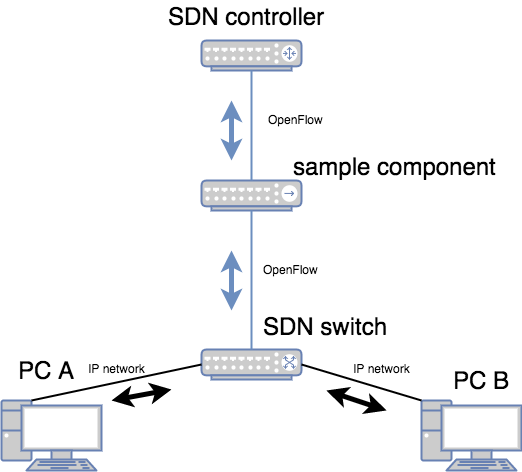
\includegraphics[width=\textwidth]{sdn_epc_flow}
\caption{Schemat podstawowej topologii sieciowej z umiejscowionym komponentem
  implementującym rozwiązanie projektowe}
\label{fig:sdn_epc_flow}
\end{figure}

Jak zostało przedstawione na Rys. \ref{fig:sdn_epc_flow} węzły końcowe
(\textit{PC N}) komunikują się ze sobą z wykorzystaniem przełącznika sieci SDN
(\textit{SDN switch}), a cały ruch pomiędzy przełącznikiem, a kontrolerem
(\textit{SDN controller}) przemieszcza się przez wspomniany komponent
implementujący rozwiązanie projektowe (\textit{sample component}).

Topologia zaprezentowana na Rys \ref{fig:sdn_epc_flow}, jak wspomniano, jest
tolopogią najbardziej podstawową, odpowiednią do wykorzystania prezentowanego
rozwiązania. Możliwe jest również, zastosowanie tego rozwiązania w bardziej
rozbudowanej sieci, składającej się z większej liczby węzłów końcowych, 
przełączników oraz kontrolerów. W takim przypadku, można zastosować kilka
instancji równlegle działającego oprogramowania (komponentu), w celu
zwiększenia wydajności systemu, rozumianego jako kilka współpracujących ze sobą
instancji. System taki, można zastosować do większych, pracujących pod większym
obciążeniem sieci. 

\section{Wybór odpowiednich technologii do implementacji systemu}

Podstawowym kryterium wyboru odpowiednich technologii do realizacji projektu
była wydajność. Wydajność jest rozumiana jako ilość pracy wykonana przez system
komputerowy w danym czasie i przy wykorzystaniu danej ilości zasobów
obliczeniowych \cite{distrforfunandprof}. Na potrzeby projektu, odpowiedni
poziom wydajności został zapewniony dzięki doborze techologi, które wspierają
koncepcję programowania współbieżnego, czyli możliwość wykonywania się
oprogramowania z wykorzytaniem wielu wątków fizycznych procesora maszyny, na
której zostało ono uruchomione. Ponadto, przy wyborze technologi, kierowano się
również natywnym wsparciem dla możliwosći dystrybucji oprogramowania na wiele
maszyn fizycznych, czyli, innymi słowy, wsparciem dla budowania systemów
rozproszonych. Możliwość rozbudowy systemu z wykorzystaniem wielu maszyn jest
kluczowa, ponieważ nawet dysponując technolgią ze wsparciem dla programowania
współbieżnego, istnieje granica dla rozbudowy zasobów sprzętowych, dlatego w
pewnym momencie koniecznym jest budowa systemu rozproszonego
\cite{distrforfunandprof}. 

Wykorzystanie technolgii, która umożliwa programowanie współbieżne oraz wspiera
budowę systemów rozporosznych, umożliwiło taką implementację projeku, która
pozwala na łatwe oraz efektywne jego skalowanie, celem zwiększenia wydajności.

Technologiami, które spełniają wszystkie wyżej wymienione wytyczne są funkcyjne
języki programowania Erlang oraz Elixir. Oba języki działają na Maszynie
Wirtualnej Erlanga (\textit{BEAM}). W rzeczywistości Elixir jest nowoczesną wersją
Erlanga, dopasowaną do dzisiejszych standardów. Oferuje on szereg nowoczesnych,
ułatwiających pracę programistyczną narzędzi, których Erlang nie posiada. W
rzeczywistości Elixir jest Erlangową aplikacją działającą na Maszynie Wirtualnej
Erlanga \cite{thebeambook}.

Maszyna Wirtualna Erlanga wprowadza model aktorów
\footnote{https://en.wikipedia.org/wiki/Actor\_model}, dzięki czemu posiada
natywne wsparcie dla programowania równoległego. Ponadto, \textit{BEAM} zapewnia
również wsparcie dla budowy systemów rozproszonych \cite{lyserlang}. Dzięki
temu, języki Erlang oraz Elixir są odpowiednie do budowy wydajnych,
niezawodnych, systemów rozproszonych. Z tych właśnie powodów, wspomniane
technologie zostały wykorzystane do budowy projektu przedstawionego w niniejszej
pracy.

\section{Algorytm detekcji ataku DDoS} \label{algorithm}

Alogrytm detekcji ataku, zaimplementowany na potrzeby opisywanego projektu
bazuje na entropii pakietów przepływających przez sieć SDN. Entropia pakietów
rozumiana jest jako ich losowość. Im większa entropia tym większa losowość
pakietów i odwrotnie \cite{mainddosarticle}. Entropia jest wyliczana na postawie
wzoru \ref{equ:entropy} \cite{mainddosarticle}.

\begin{equation}
H = -\sum_{i=1}^{n}p_{i}\log_{}p_{i}
\label{equ:entropy}
\end{equation}
gdzie $H$ oznacza wartość entropii, $n$ liczbę pakietów (tzw. rozmiar okna),
a $p_{i}$ wartość prawdopodbieństwa wystąpienia poszczególnego pakietu.

Wspomniany rozmiar okna jest defininowany jako ilość pakietów, dla których
została obliczona entropia. Rozważając przypadek dla okna o rozmiarze 50, przy
założeniu, że każdy element okna wystąpił dokładnie jeden raz, wartośc entropi
obliczonej zgodnie ze wzorem \ref{equ:entropy} wyniesie 1,70. Natomiast w
przypadku, gdy jeden z elementów okna pojawi się dokładnie dziesięć razy, a
pozostałe 40 elementów tylko raz, entropia wyniesie 1,47.

Przedstawiona zależność entropii i losowości pakietów została wykorzystana do
wykrywania ataku DDoS. Atak DDoS zazwyczaj skupia się na jednym, wybranym węźle
końcowym, czyli w przypadku ataku większość pakietów w sieci zawiera jeden,
konkretny adres docelowy. W takiej sytuacji losowość pakietów w sieci spada, a
co za tym idzie, spada również entropia. Bazując na tym fakcie, można ustalić
limit wartości entropii poniżej którego, uznaje się, że w sieci nastąpił atak
DDoS. 

Algorytm zaimplementowany na potrzeby opisywanego projektu analizuje adresy
docelowe pakietów \textit{IP} przepływających przez sieć, tj. zlicza ilość
wystąpień każdego adresu docelowego zawartego w badanych pakietach \textit{IP}.
Gdy ilość przeanalizwanych pakietów jest równa rozmiarowi okna obliczana jest 
entropia. W tym celu wykorzystywane są równania: \ref{equ:entropy},
\ref{equ:window} \cite{mainddosarticle} oraz \ref{equ:packet_prob}
\cite{mainddosarticle}.

\begin{equation}
W = \{(x_{1},y_{1}),(x_{2},y_{2}),(x_{3},y_{3}),...\}
\label{equ:window}
\end{equation}

\begin{equation}
p_{i} = \frac{y_{i}}{n}
\label{equ:packet_prob}
\end{equation}

Równanie \ref{equ:window} przedstawia reprezentację okna ($W$), gdzie $x_{i}$
oznacza dany docelowy adres \textit{IP}, a $y_{i}$ liczbę jego wystąpień w danym
oknie. Równanie \ref{equ:packet_prob} pozwala wyliczyć prawdopodobieństwo
danego pakietu ($p_{i}$), gdzie $y_{i}$ oznacza liczbę wystąpień danego adresu
\textit{IP}, a $n$ liczbę wszystkich pakietów w oknie ($W$).
Jeśli obliczona wartość entropii dla określonej liczby okien z rzędu
(rekomendowana liczba okien  wynosi 5 \cite{mainddosarticle}) jest mniejsza niż
zadana wartość, uznaje się, że w sieci nastąpił atak. 

\section{Aplikacja wykrywania ataku DDoS}

Aplikacja \textit{sdn\_epc} \footnote{https://github.com/mkacper/sdn\_epc}
(\textit{Software Defined Networking Elixir Pseudo Controller}) została w
głównej mierze wykonana przy użyciu języka programowania Elixir, aczkolwiek
wykorzstuje również kod napisany w Erlangu (głównie do interakcji z zewnętrznymi
Erlangowymi bibliotekami). Użycie dwóch języków jednocześnie było możliwe,
ponieważ, jak wspomniano we wcześniejszym rozdziale, oba te języki finalnie są
kompilowne do tego samego kodu binarnego i wykonują się na tej samej maszynie
wirtualnej (\textit{BEAM}). Ponadto, kompilator Elixira potrafi również
kompilować kod Erlanga.

\subsection{Zasada działania aplikacji}

Jak przedstawiono na Rys. \ref{fig:sdn_epc_flow} strona
\pageref{fig:sdn_epc_flow} aplikacja \textit{sdn\_epc} została zaprogramowana
jako osobny komponent, działający na osobnej maszynie, połączony bezpośrednio z
przełącznikami oraz z kontrolerm sieci SDN. Komponenty te komunikują się ze
sobą z wykorzystaniem protokołu \textit{OpenFlow}. W przedstawionej konfiguracji,
cały ruch sieciowy pomiędzy przełącznikami, a kontorelerem przepływa przez
komponent \textit{sdn\_epc}. Umożliwienie połączenia systemu Elixirowego z
komponentami sieciowym, z wykorzystaniem \textit{OpenFlow} wymaga umiejętności
obsługi tego protokołu przez aplikację \textit{sdn\_epc}. W tym celu
wykorzystane zostały Erlangowe biblioteki \textit{of\_protocol}
\footnote{https://github.com/FlowForwarding/of\_protocol} oraz
\textit{ofs\_handler} \footnote{https://github.com/FlowForwarding/ofs\_handler}.

Przepływający przez komponent \textit{sdn\_epc} ruch \textit{OpenFlow} jest
analizowany na potrzeby algorytmu opisanego w rozdziale \ref{algorithm}.
Analizowane są wiadomości \textit{PACKET\_IN} protokołu \textit{OpenFlow}, a
konkretnie docelowe adresy pakietów \textit{IP} przesyłanych jako część
wiadomości \textit{PACKET\_IN}. Wyniki zapisywane są w rozproszonej bazie danych
(\textit{Mnesia}) \footnote{hhttp://erlang.org/doc/apps/mnesia/index.htm}
dostarczanej razem ze standardową dystrybucją Erlanga. Następnie, zapisane
wyniki wykorzystywane są do działania wspomnianego algorytmu.

\subsection{Wydajność aplikacji}

Architektura aplikacji \textit{sdn\_epc} uwzględnia możliwosci jakie daje
Maszyna Wirtualna Erlanga w zakresie programowania równoległego oraz dystrybucji
oprogramowania na wiele węzłów. Dzięki wsparciu dla programowania równoległego
aplikacja \textit{sdn\_epc} może w tym samym czasie obsługiwać wiele (w
rzeczywistości tyle ile wątków może obsłużyc maszyna, na której działa
aplikacja) podłączonych do niej przełączników sieci SDN. \textit{BEAM} wprowadza
koncepcję procesów, w kontekście których, wykonuje się każdy kawałek
Erlangowego/Elixirowego kodu. Koncepcja ta jest podobna do koncepcji procesów
systemowych - wykonują się one na wszystkich procesorach (jeden proces na
jednym procesorze w tym samym czasie), ale mają znacznie mniejszy narzut w
kontekście zużycia zasobów systemowych niż tradycyjne procesy \cite{progelixir}.
Wykorzystując koncepcję procesów, kod odpowiedzialny za obsługę przełączników
podłączonych do aplikacji wykonuje się w osobnym procesie dla każdego z
przełączników. Innym słowy, każdy przełącznik jest obsługiwany przez osobny,
dedykowany dla niego proces, co umożliwa jednoczesną obsługę wielu
przełączników.

Aplikacja \textit{sdn\_epc} może działać w klastrze, dzięki czemu możliwe jest
zwiększenie jej wydajności. Do działania w klastrze aplikacja wykorzystuje
wbudowany w \textit{BEAM}'a mechanizm zwany \textit{Erlang Distributed}
\footnote{http://erlang.org/doc/reference\_manual/distributed.html}. Mechnizm
ten umożliwa komunikowanie się ze sobą wielu węzłów (Maszyn Wirtualnych
Erlanga) \cite{erldocs}. Dzięki wspomnianej koncepcji procesów rozproszenie
oprogramowania na wiele węzłów nie stanowi problemu, ponieważ z punktu widzenia
Erlangowego systemu nie ma znaczenia, na którym węźle wykonuje się dany proces
(procesy komunikują się w ten sam sposób, niezależnie od węzła na którym
działają \cite{erldocs}). Jednkaże, w przypadku działania w aplikacji
\textit{sdn\_epc} w klastrze, pojawił się problem z synchronizacją stanu (danych
zapisywanych na potrzeby algorytmu do wykrywania ataku DDoS) pomiędzy węzłami.

%OK jak działą, switch <-> sdn_Epc <-> ctrl, openflow
%OK ze analizuje PACKET_IN
%OK że jest switch per procs
%OK że da się klastrować
% że problem z synchronizacją stanu, mnesia

\chapter{Weryfikacja rozwiązania}

W celu weryfikacji poprawności działania zaimplementowanego systemu zostały
wykonane serie testów. System został przetestowany pod kątem sprawdzenia
podstawowych założeń projektowych tj. poprawności wykrywania anomali związanych
z natężeniem ruchu w obsługiwanej sieci oraz możliwości skalowania
aplikacji \textit{sdn\_epc} w celu zwiększenia wydajności systemu.
Przeprowadzenie testów wymagało przygotowania odpowiednich scenariuszy testowych,
zestawienia dedykowanych topolgi sieciowych oraz stworzenia rozwiązań
pozwalających na zebranie własciwych danych z testowanego systemu. Analiza
tychże wyników pozwoliła na stwierdzenie, czy i w jakim stopniu założenia
projektowe zostały spełnione. Niniejszy rozdział szczegółowo opisuje
poszczególne przypadki testowe oraz prezentuje analizę uzyskanych wyników.

\section{Test działania implementacji algorytmu}

Aby stwierdzić, czy zaimplementowany algorytm (rozdział \ref{algorithm} strona
\pageref{algorithm}) w aplikacji \textit{sdn\_epc} spełnia swoją rolę tzn.
pozwala wykryć atak DDoS w sieci SDN zostały przeanalizowane wartości entropii
obliczone za pomocą tegoż właśnie algorytmu w dwóch różnych przypadkach
testowych, z których każdy wykorzystywał nieco inną konfigurację testową
topologi sieciowej, jak również samej aplikacji \textit{sdn\_epc}. Przetestowane
zostały przypadki, gdy:  
\begin{enumerate}
  \item Ruch wygenerowany w sieci testowej był obsługiwany tylko przez jeden
    węzeł aplikacji \textit{sdn\_epc}.
  \item Ruch wygenerowanych w sieci testowej był obsługiwany przez wiele węzłów
    aplikacji \textit{sdn\_epc} działających w klastrze.
\end{enumerate}
Wykorzystanie takich właśnie przypadków testowych umożliwiło sprawdzenie
poprawności implementacji algorytmu zarówno w przypadku działania systemu jako
pojedynczy węzeł aplikacji \textit{sdn\_epc}, jak również w przypadku, gdy
system działał w klastrze. Drugi przypadek jest znacznie bardziej złożony,
ponieważ rozproszenie procesu obliczania algorytmu na wiele węzłów wprowadza
dodatkowe komplikacje, związane z synchronizacją stanu pomiędzy węzłami.

\subsection{Przypadek testowy z wykorzystaniem jednego węzła aplikacji
  \textit{sdn\_epc}} \label{entropy_one_node}

Schemat topologii sieciowej wykorzystanej w przypadku, gdy tylko jeden węzeł
aplikacji jest zaangażowany w przetwarzenie ruchu został przedstawiony na
Rys. \ref{fig:entropia_scheme}.

\begin{figure}[h]
\centering
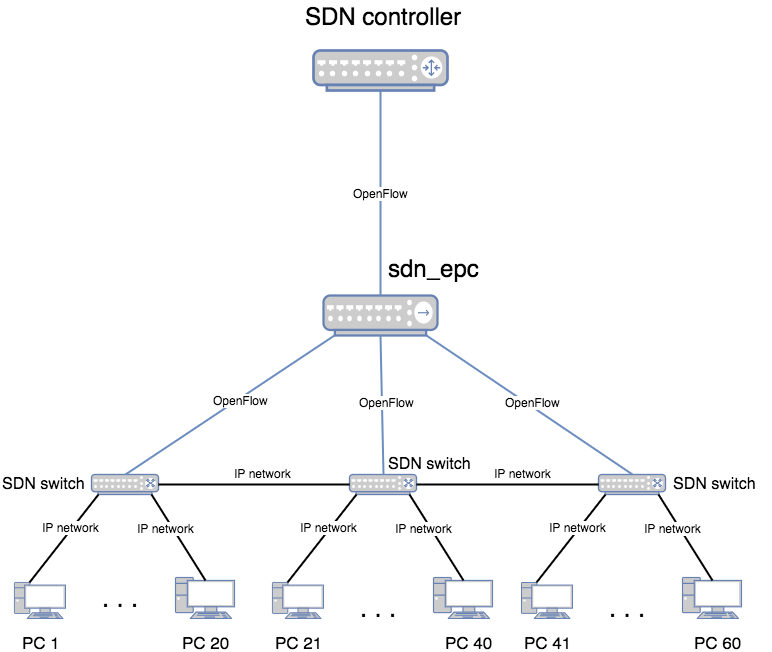
\includegraphics[width=\textwidth]{entropia_scheme}
\caption{Schemat topologii sieciowej z wykorzystaniem jednego węzła aplikacji
  \textit{sdn\_epc}}
\label{fig:entropia_scheme}
\end{figure}

W topologii przedstawionej na Rys. \ref{fig:entropia_scheme} wszystkie
przełączniki obsługujące ruch pomiędzy węzłami końcowymi (\textit{PC N})
komunikują się z kontrolerem (\textit{SDN controller}) poprzez jeden węzeł
aplikacji \textit{sdn\_epc}. Wykorzystując taką konfigurację sieci, tylko jeden
węzeł \textit{sdn\_epc} przetwarza wiadomości \mbox{\textit{PACKET\_IN}}
protokołu \textit{OpenFlow}, wymieniane pomiędzy poszczególnymi przełącznikami,
a kontrolerem, w celu obliczenia entropii pakietów przesyłanych w sieci.

Jeśli algorytm został poprawnie zaimplementowany to wartość entropii,
obliczonej za jego pomocą, powinna maleć wzraz ze spadkiem losowości pakietów
przesyłanych w sieci testowej. Innymi słowy, im więcej pakietów w sieci jest
adresowanych do jednego, konkretnego węzła końcowego, tym mniejsza będzie wartość
obliczonej entropii.

W celu sprawdzenia czy wspomiana zależność została spełniona, koniecznym było
zaprojektowanie odpowiedniego scenariusza testowego. Scenariusz ten opierał się
na środowisku testowym przedstawionym na Rys. \ref{fig:entropia_tech}.

\begin{figure}[h]
\centering
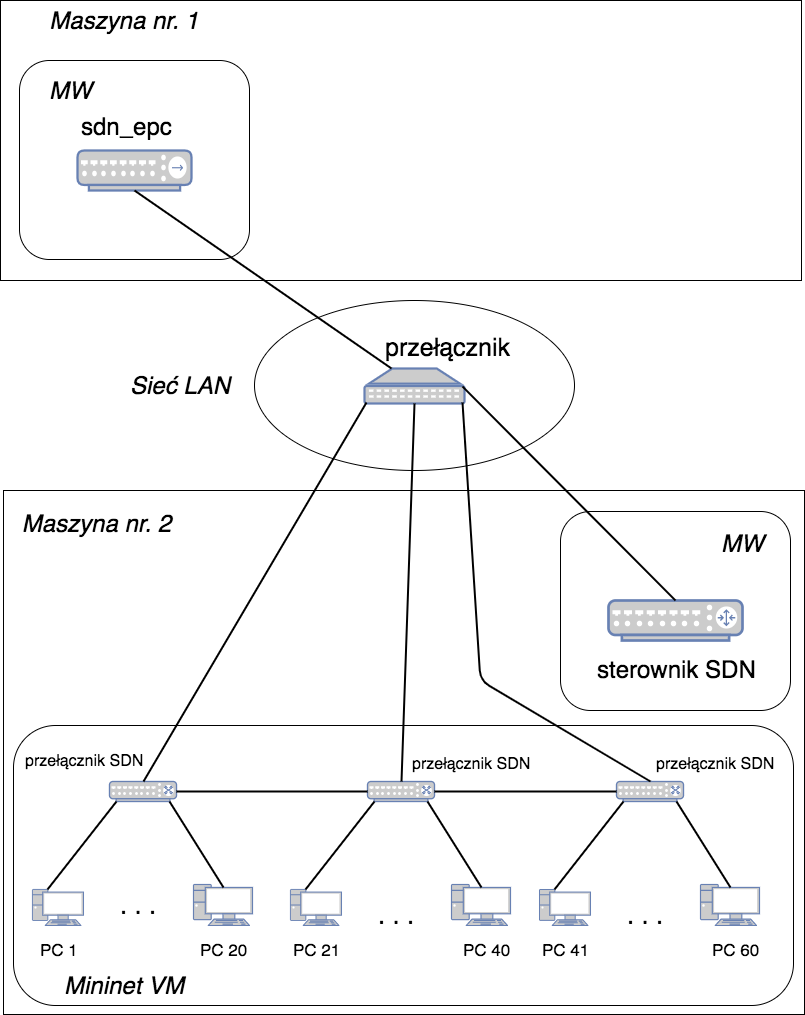
\includegraphics[height=11cm]{entropia_tech}
\caption{Środowisko testowe z wykorzystaniem jednego węzła aplikacji
  \textit{sdn\_epc}}
\label{fig:entropia_tech}
\end{figure}

Jak przedstawiono na Rys. \ref{fig:entropia_tech} toplogia sieciowa została
zestawiona z użyciem dwóch maszyn fizycznych, na których zostały zwirtualizowane
niezbędne komponenty testowe. Każdy z komponentów, za wyjątkiem przełącznika
sieci \textit{LAN} (\textit{switch}), został uruchomiony na dedykowanej maszynie
wirtualnej. Jako środowisko do wirtualizacji zostało wykorzystane oprogramowanie
\textit{VirtualBox \footnote{https://www.virtualbox.org}}. Maszyny wirtualne
komunikowały się ze sobą z wykorzystaniem sieci \textit{LAN}.

Przełączniki sieci SDN (\textit{SDN switch}) oraz węzły końcowe (\textit{PC
  N}) były emulowane na dedykowanej maszynie wirtualnej za pomocą oprogramowania
\textit{Mininet \footnote{http://mininet.org}}. Wykorzystane w teście
przełączniki to domyślne przełączniki używane przez oprogramowanie
\textit{Mininet}, które działają na bazie oprogramowania
\textit{Open vSwitch \footnote{http://openvswitch.org}} \cite{mininetwiki}.
\textit{SDN controller}, pełniący funkcję kontrolera w testowej topologii,
korzystał z oprogramowania zbudowanego z wykrzystaniem framework'a
\textit{Ryu \footnote{https://osrg.github.io/ryu}}. Maszyny wirtualne dedykowane
dla \textit{sdn\_epc} i \textit{SDN controller} działały pod kontrolą systemu
operacyjnego \textit{Ubuntu \footnote{https://www.ubuntu.com}}.

W celu poprawnego działania algorymu musi zostać spełnione założenie: dla
każdego nowego połączenia (adres źródłowy/docelowy, port źródłowy/docelowy oraz
protokół; na potrzeby ninejszej pracy wykorzystano tylko adres
docelowy/źródłowy) kontroler sieci SDN instaluje nowy przepływ w przełączniku
sieci SDN \cite{mainddosarticle}. Przy takim założeniu, każde nowe połączenie w
sieci wygeneruje wiadomość \textit{PACKET\_IN}, która następnie zostanie
przeanalizowana przez węzeł \textit{sdn\_epc}. Aby spełnić to założenie należało
zmodyfikować logikę przełącznika zaimplementowaną w kontrolerze. Modyfikacja
wymagała przeprogramowania \textit{Python}'owego skrytpu odpowiedzialnego za
implementację logiki przełącznika w oprogramowaniu kontrolera \cite{ryupage}.

Scenariusz testowy zakładał przeprowadzenie kilku prób, podczas których w sieci
były generowane ataki DDoS o różnej sile. Podczas każdej próby została zmierzona
średnia wartość entropii obliczonej za pomocą zaimplementowanego algorytmu.
Wykonane zostały cztery próby z atakami o sile odpowiednio: 0\%, 30\%, 60\% oraz
90\%. Siła każdego ataku została obliczona na podstawie wzoru
\ref{equ:ddos_power} \cite{mainddosarticle}

\begin{equation}
R = \frac{P_{a}}{P_{n}} \cdot 100\%
\label{equ:ddos_power}
\end{equation}
gdzie R oznacza siłę ataku, $P_{a}$ pakiety atakujące, natomiast $P_{n}$ pakiety
tła.

Pakiety tła rozumiane są jako pakiety
\textit{IP \footnote{https://tools.ietf.org/html/rfc791\#section-3.1}} wysyłane
do losowo wybranych węzłów końcowych w stałych odstępach czasowych. Pakiety
atakujące oznaczają pakiety \textit{IP}, które zawierają losowe adresy źródłowe
oraz są wysyłane do konkretnego węzła końcowego w 4-krotnie krótszych odstępach
czasowych niż pakiety tła. 

Podczas każdej próby wybrane węzły końcowe generowały pakiety tła oraz
pakiety atakujące (jeden węzeł generował jeden typ pakietów). Do generowania
pakietów została wykorzystana biblioteka języka \textit{Python} o nazwie
\textit{ Scapy \footnote{http://www.secdev.org/projects/scapy}}. Szczegółowe
dane opisujące każdą z prób zostały przedstawione w Tab. \ref{tab:entropy}.

\begin{table}[h!]
\centering
\begin{tabular}{ |c|c|c|c|c| } 
 \hline
 R & $P_{n}$ & $P_{a}$ & interwał $P_{n}$ & interwał $P_{a}$ \\
 \hline
 0\% & 3000 & 0 & 20ms & 5ms \\ 
 \hline
 30\% & 3000 & 900 & 20ms & 5ms \\ 
 \hline
 60\% & 3000 & 1800 & 20ms & 5ms \\ 
 \hline
 90\% & 3000 & 2700 & 20ms & 5ms \\ 
 \hline
\end{tabular}
\caption{Parametry prób testowych z wykorzystaniem jednego węzła aplikacji
  \textit{sdn\_epc}} 
\label{tab:entropy}
\end{table}

Warto zaznaczyć, że średnio 3,4\% wszystkich pakietów z danej próby nie dotarło
do aplikacji \textit{sdn\_epc}. Wydaje się, że nie powinno wpłynąć to znacząco
na uzyskane wyniki, jednak ze względu na fakt, że przeprowadzenie tego typu
testów wymaga znacznych zasobów obliczeniowych, do których dostęp nie jest
ogólnodostępny, wpływ wspomianego zjawiska nie został naukowo zbadany w
niniejszej pracy.

Na wykresie \ref{plot:entropy} przedstawiono średnią wartość entropii,
obliczonej przez aplikację \textit{sdn\_epc} przy użyciu zaimplementowanego w
niej algorytmu, dla poszczególnych prób testowych.

\begin{figure}[h]
\centering
\begin{tikzpicture}
\begin{axis}[
    xlabel={Siła ataku [\%]},
    ylabel={Średnia wartośc entropii},
    xmin=0, xmax=100,
    ymin=0.7, ymax=1.2,
    xtick={0,20,40,60,80,100},
    ytick={0.7,0.8,0.9,1,1.1,1.2},
    legend pos=outer north east,
    ymajorgrids=true,
    grid style=dashed,
]
 
\addplot[
    color=blue,
    mark=square,
    ]
    coordinates {
    (0,1.164)(30,1.025)(60,0.891)(90,0.748)
    };
    \legend{jeden węzeł \textit{sdn\_epc}}
 
\end{axis}
\end{tikzpicture}
\caption{Średnia wartość entropii w zależności od siły ataku DDoS}
\label{plot:entropy}
\end{figure}
\newpage

Zależność entropii od siły ataku, przedstawiona na wykresie \ref{plot:entropy},
jest taka, jak przewidywano. Wzraz ze wzrostem siły ataku wartość entropii
maleje, ponieważ im większa siła ataku, tym większy procent wszystkich pakietów
w sieci trafia do jednego, atakowanego, węzła końcowego. W związku z tym,
losowość poszczególnych pakietów spada, tym samym powodując spadek entropii
pakietów w sieci.

Bazując na przestawionych wynikach i ich analizie, można stwiedzić, że alogorytm
służacy do wykrywania ataku DDoS, został poprawnie zaimplementowany w aplikacji
\textit{sdn\_epc} i umożliwa wykrycie tego typu anomali. 

\subsection{Przypadek testowy z wykorzystaniem kilku węzłów aplikacji
  \textit{sdn\_epc} działających w klastrze} \label{entropy_multi_node}

Schemat topologii sieciowej wykorzystanej w przypadku, gdy kilka węzłów
aplikacji \textit{sdn\_epc} działających w klastrze obsługuje ruch w sieci
został zaprezentowany na Rys. \ref{fig:entropia_multi_scheme}.
\newpage

\begin{figure}[h]
\centering
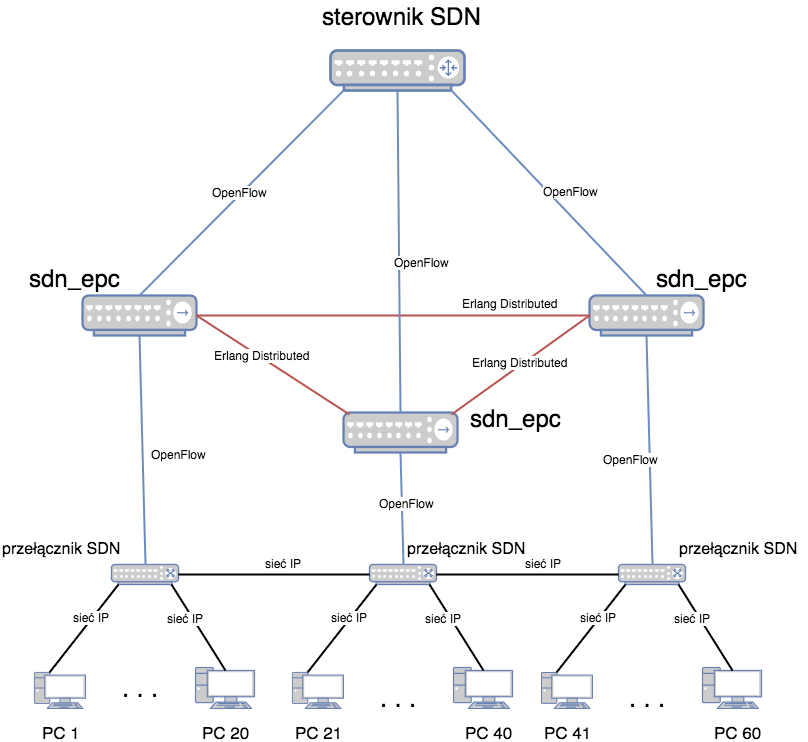
\includegraphics[width=\textwidth]{entropia_multi_scheme}
\caption{Schemat topologii sieciowej z wykorzystaniem trzech węzłów aplikacji
  \textit{sdn\_epc} działających w klastrze}
\label{fig:entropia_multi_scheme}
\end{figure}

Topologia przedstawiona na Rys. \ref{fig:entropia_multi_scheme} jest bardzo
podobna do przedstawionej na Rys. \ref{fig:entropia_scheme} na stronie
\pageref{fig:entropia_scheme}. W tym przypadku każdy przełącznik w sieci
komunikuje się z kontrolerem poprzez dedykowany węzeł aplikacji
\textit{sdn\_epc}, a więc w klastrze działa dokładnie tyle węzłów
\textit{sdn\_epc} ile jest przełączników w sieci. Każdy węzeł aplikacji obsłguje
tylko jeden przełącznik. Najważniejszą różnicą, względem przypadku, gdy tylko
jeden węzeł aplikacji obsługuje wszystkie przełączniki w sieci, jest 
rozproszenie procesu obliczania entropii na wiele węzłów \textit{sdn\_epc}.

W związku z tym, że rozposzenie procesu obliczania entropii na wiele węzłów,
wprowadziło szereg komplikacji, które należło uwzględnić, aby poprawnie ją
obliczyć, zostały przeprowadzene dokładnie takie same próby testowe, jak opisano
w sekcji \ref{entropy_one_node} ale z wykorzystaniem innej topologii testowej.
Przeprowadzenie bliźniaczych prób pozwoliło porównać wyniki, tj. wartości
entropii, w przypadku obliczania jej z użyciem jednego (patrz wykres
\ref{plot:entropy} strona \pageref{plot:entropy}) oraz kilku węzłów
\textit{sdn\_epc}. Takie porównanie pozwoliło ustalić, czy zaimplementowany
algorytm działa poprawnie również w przypadku rozproszenia procesu obliczania
entropii.

Środowisko przygotowane na potrzeby przeprowadzenia prób testowych, z
wykorzystaniem kilku węzłow \textit{sdn\_epc} przedstawiono na Rys.
\ref{fig:entropy_multi_tech}.

\begin{figure}[h]
\centering
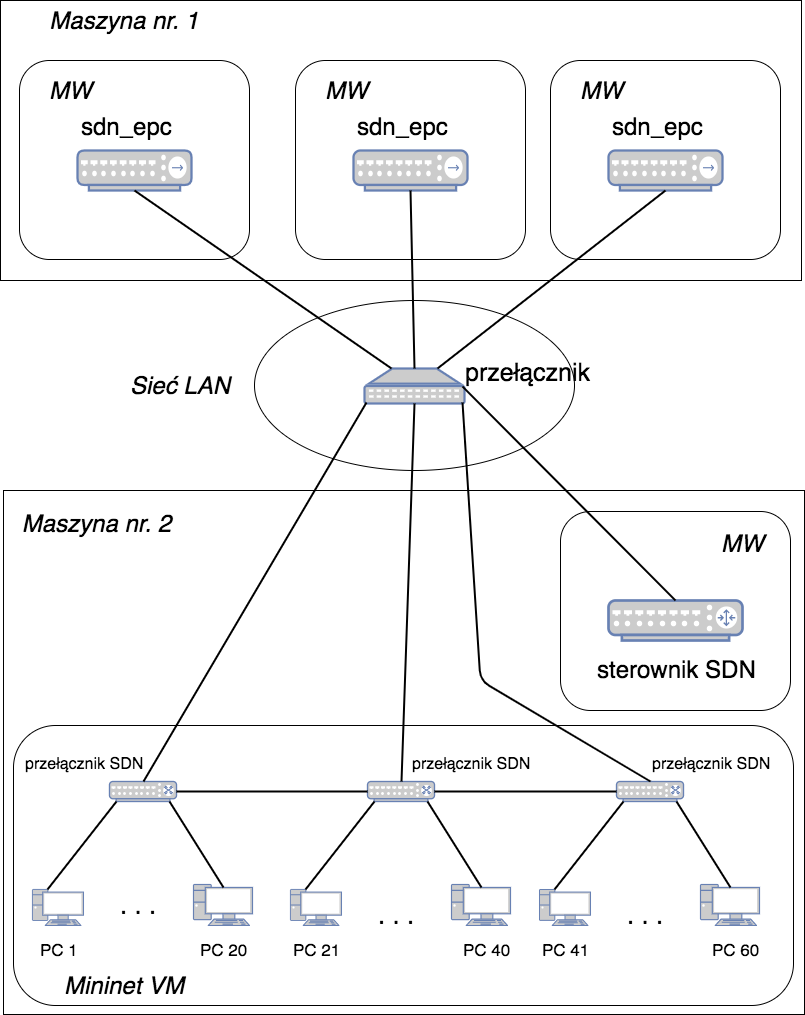
\includegraphics[height=11cm]{entropy_multi_tech}
\caption{Środowisko testowe z wykorzystaniem trzech węzłów aplikacji
  \textit{sdn\_epc} działających w klastrze}
\label{fig:entropy_multi_tech}
\end{figure}

Testowa topologia sieciowa przedstawiona na Rys. \ref{fig:entropy_multi_tech}
została zbudowana z takich samych komponentów i wykorzystując dokładnie takie
same rozwiązania i technologie jak przedstawiono na Rys. \ref{fig:entropia_tech}
strona \pageref{fig:entropia_tech} oraz opisano w sekcji \ref{entropy_one_node}.

W celu zmierzenia średniej wartości entropii z wykorzystaniem wielu węzłów
aplikacji \textit{sdn\_epc} przeprowadzono takie same próby testowe jak opisano
w Tab. \ref{tab:entropy} strona \pageref{tab:entropy}. Uzyskane wyniki zostały
przedstawione na wykresie \ref{plot:entropy_multi_node} wraz z wynikami
pozyskanymi podczas prób z wykorzystaniem jednego węzła \textit{sdn\_epc}, aby
umożliwić porównanie wyników otrzymanych z użyciem dwóch różnych topolgii
sieciowych.

\begin{figure}[h]
\centering
\begin{tikzpicture}
\begin{axis}[
    xlabel={Siła ataku [\%]},
    ylabel={Średnia wartośc entropii},
    xmin=0, xmax=100,
    ymin=0.7, ymax=1.2,
    xtick={0,20,40,60,80,100},
    ytick={0.7,0.8,0.9,1,1.1,1.2},
    legend pos=outer north east,
    ymajorgrids=true,
    grid style=dashed,
]

\addplot[
    color=blue,
    mark=square,
    ]
    coordinates {
    (0,1.164)(30,1.025)(60,0.891)(90,0.748)
    };
    \addlegendentry{jeden węzeł \textit{sdn\_epc}}

\addplot[
    color=red,
    mark=*,
    ]
    coordinates {
    (0,1.171)(30,1.027)(60,0.903)(90,0.746)
    };
    \addlegendentry{trzy węzły \textit{sdn\_epc}}

\end{axis}
\end{tikzpicture}
\caption{Średnia wartość entropii dla różnych konfiguracji testowych w
  zależności od siły ataku DDoS}
\label{plot:entropy_multi_node}
\end{figure}

Analizując wykres \ref{plot:entropy_multi_node} można zauważyć, że wartości
obliczonej entropii w obu przypadkach są niemal identyczne. Widoczne różnice
mogą być spowodowane przez straty pakietów w sieci (średnio w każdej próbie, z
wykorzystaniem topologii przedstawionej na Rys. \ref{fig:entropia_multi_scheme},
2,9\% wszystkich pakietów nie dotarło do węzła \textit{sdn\_epc}) oraz
niedoskonałością generatora losowego wykorzystanego do generowania adresów
docelowych dla pakietów \textit{IP} użytych do generowania ruchu podczas prób
testowych. Ze względu na ograniczenia techniczne, związane z dostępem do zasobów
obliczeniowych niezbędnych do przeprowadzenia testów, zjawiska te nie zostały
naukowo zbadane w niniejszej pracy. Jednakże różnice w wynikach są  na tyle
małe, że można uznać, iż zaimplementowany algorytm, służacy do wykrywania ataku
DDoS, działa poprawnie zarówno w systemie rozproszonym jak i z wykorzystaniem
jednego węzła \textit{sdn\_epc}.

\section{Test skalowalności horyzontalnej}

Celem weryfikacji skalowalności zaproponowanego rozwiązania zostały
przeprowadzone serie testów, podczas których zmierzono zużycie zasobów
obliczeniowych, a konkretnie czas zajętości procesora, wykorzystanych na
potrzeby przetwarzania ruchu sieciowego przez węzeł aplikacji \textit{sdn\_epc}.
Testy wykonano z wykorzystaniem dwóch różnych konfiguracji testowych:
\begin{enumerate}
  \item \label{tc:cluster_1} Ruch wygenerowany w sieci testowej był obsługiwany
    przez jeden węzeł aplikacji \textit{sdn\_epc} działający w klastrze.
  \item \label{tc:cluster_n} Ruch wygenerowany w sieci testowej był obsługiwany
    przez wiele węzłów aplikacji \textit{sdn\_epc} działających w klastrze.
\end{enumerate}

Porównanie średnich wartości czasu zajętości procesora pozwoliło stwierdzić,
czy dodanie kolejnych węzłów \textit{sdn\_epc} do klastra, celem rozłożenia
ruchu (obciążenia) na inne węzły, obniżyło zużycie zasobów przez pojedynczy
węzeł. Podczas każdej z prób testowych pomiary zostały przeprowadzone na tym
samym węźle aplikacji \textit{sdn\_epc}.

Schematy przedstawione na Rys. \ref{fig:cluster_scheme_single_node} oraz
Rys. \ref{fig:cluster_scheme_multi_node} prezentują odpowiednio przypadki
testowe opisane w Ad. \ref{tc:cluster_1} oraz Ad. \ref{tc:cluster_n}. Węzeł
na którym dokonano pomiarów został zaznaczony czerwonym okręgiem.
\newpage

\begin{figure}[h]
\centering
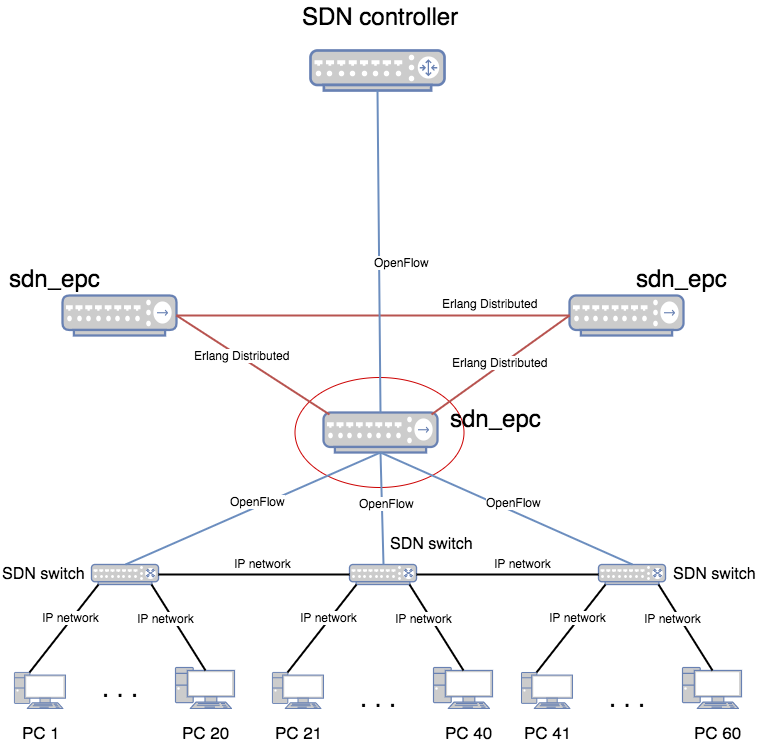
\includegraphics[width=\textwidth]{cluster_scheme_single_node}
\caption{Schemat topologii sieciowej z wykorzystaniem jednego węzła aplikacji
   \textit{sdn\_epc}, do obsługi ruchu sieciowego, działającego w klastrze}
\label{fig:cluster_scheme_single_node}
\end{figure}
\newpage

\begin{figure}[h]
\centering
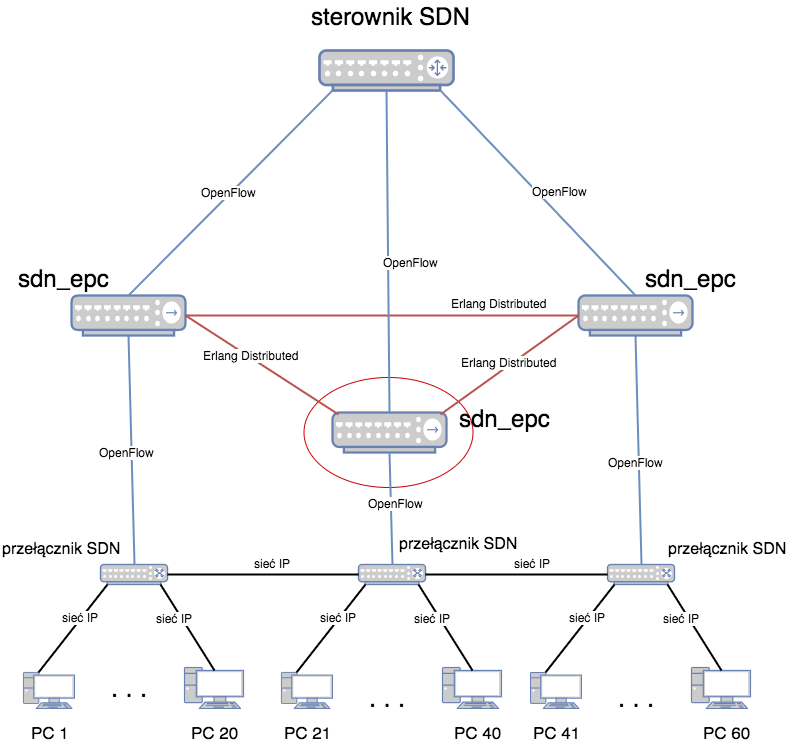
\includegraphics[width=\textwidth]{cluster_scheme_multi_node}
\caption{Schemat topologii sieciowej z wykorzystaniem trzech węzłów aplikacji
  \textit{sdn\_epc}, do obsługi ruchu sieciowego, działających w klastrze}
\label{fig:cluster_scheme_multi_node}
\end{figure}

Rozwiązanie przedstawione na Rys. \ref{fig:cluster_scheme_single_node}
wykorzystuje klaster węzłów \textit{sdn\_epc}, podczas gdy tylko jeden węzeł
jest zaangażowany w obsługę ruchu sieciowego. Takie rozwiązanie nie powinno być
wdrożone w jakimkolwiek systemie produkcyjnym, ponieważ budowanie klastra, w
którym używany jest tylko jeden węzeł w większości przypadków nie ma logicznego
uzasadnienia. Rozwiązanie to zostało wykorzystane na potrzeby niniejszej pracy
inżynierskiej tylko i wyłącznie z powodu niedoskonałości aplikacji
\textit{sdn\_epc}. W obecnej wersji aplikacji nie zostały dokonane żadne
optymalizacje związane z synchronizacją i dostępem do stanu pomiędzy węzłami. Z
powodu braku wspomnianych optymalizacji działanie aplikacji w klastrze wprowadza
znaczny narzut obliczeniowy. Użycie wymienionego wyżej rozwiązania pozwoliło
niejako ująć rzeczony narzut w pomiarach zużycia zasobów obliczeniowych dla
przypadku, gdy ruch sieciowy jest obsługiwany przez jeden węzeł
\textit{sdn\_epc}. Innymi słowy, różnica pomiędzy zmierzonym zużyciem zasobów
obliczeniowych dla wspominanych przypadków testowych nie zawiera wyż.wym.
narzutu. 

Architektura środowiska wykorzystanego na potrzeby testu jest dokładnie taka
sama jak przedstawiono na Rys. \ref{fig:entropy_multi_tech} strona
\pageref{fig:entropy_multi_tech} oraz opisano w sekcji \ref{entropy_multi_node}.
Wykorzystuje ona te same komponenty, rozwiązania oraz technologie jak te, które
opisano w wyż.wym. sekcji.

Scenariusz testowy, który wykorzystano podczas dwóch przeprowadzonych prób
testowych (Ad. \ref{tc:cluster_1} oraz Ad. \ref{tc:cluster_n} strona
\pageref{tc:cluster_1}) zakładał wykorzystanie odpowiednio logicznych topologii
sieciowych przedstawionych na Rys. \ref{fig:cluster_scheme_single_node} oraz
Rys. \ref{fig:cluster_scheme_multi_node}. Podczas każdej z prób wybrane węzły
końcowe wygenerowały 6000 pakietów tła (wyjaśnienie sekcja
\ref{entropy_multi_node}). Następnie na wybranym węźle aplikacji
\textit{sdn\_epc} (tym samym dla każdej próby) zmierzono średni czas zajętości 
procesora. Pomiarów dokonano z wykorzystaniem oprogramowania \textit{sysstat
  \footnote{http://sebastien.godard.pagesperso-orange.fr}}. Wyniki obu prób
przedstawiono na Rys. \ref{plot:cpu_usage}.

\begin{figure}[h]
\centering
\begin{tikzpicture}
\begin{axis}[
xbar,
width=10cm, height=3.5cm, enlargelimits=0.5,
xlabel={Średni czas zajętości procesora [\%]},
symbolic y coords={{1 węzeł sdn\_epc},{3 węzły sdn\_epc}},
ytick=data,
nodes near coords, nodes near coords align={horizontal},
]
\addplot coordinates {(35.30,{1 węzeł sdn\_epc}) (17.16,{3 węzły sdn\_epc})};
\end{axis}
\end{tikzpicture}
\caption{Średni czas zajętości procesora dla różnych konfiguracji testowych
  (rozmiarów klastra)}
\label{plot:cpu_usage}
\end{figure}

Na Rys. \ref{plot:cpu_usage} wyraźnie widać, że dla przypadku testowego, gdy
wygenerowany ruch sieciowy był obsługiwany przez 3 węzły \textit{sdn\_epc}
zużycie zasobów znacząco zmalało, względem próby, podczas której cały ruch
siecowy obsługiwał tylko jeden węzeł \textit{sdn\_epc}. Zużycie zasobów nie
zmalało dokładnie 3-krotnie, ponieważ działanie w aplikacji w klastrze wprowadza
dodatkowy narzut związany m.in. z rywalizacją węzłów o dostęp do stanu, który
jest niezbędny do ich poprawnego działania. Podsumowując wykres
\ref{plot:cpu_usage} dowodzi, że aplikację \textit{sdn\_epc} można skalować
horyzontalnie, co przynosi wymierne korzyści w postaci zwiększenia wydajności
całego rozwiązania, opisanego w niniejszej pracy.

\chapter{Podsumowanie}

\begin{thebibliography}{99}
\bibitem{mainddosarticle} 
S. M. Mousavi, M. St-Hilarie,
''Early Dedection of DDoS Attacks against SDN Controllers'',
s. 77-81, 2015

\bibitem{distrforfunandprof} 
M. Takada,
''Distributed systems for fun and profit'',
\\\texttt{http://book.mixu.net/distsys/single-page.html} (dokument
elektroniczny, stan na dzien 13.12.2017)

\bibitem{thebeambook} 
E. Stenman,
''The BEAM book'',
\\\texttt{https://happi.github.io/theBeamBook/} (dokument elektroniczny, stan na
dzień 13.12.2017)

\bibitem{lyserlang} 
F. Hebert,
''Learn You Some Erlang for great good!'',
\\\texttt{http://learnyousomeerlang.com/content} (dokument elektroniczny, stan
na dzień 13.12.2017)

\bibitem{ryupage}
Official Ryu site,
\\\texttt{http://osrg.github.io/ryu/} (dokument elektroniczny, stan
na dzień 16.12.2017)

\bibitem{progelixir} 
D. Thomas,
''Programming Elixir 1.2'',
2016 

\bibitem{erldocs}
Official Erlang Documentation,
\\\texttt{http://erlang.org/doc/} (dokument elektroniczny, stan
na dzień 16.12.2017)
\end{thebibliography}

\newpage
\listoftables

\newpage
\listoffigures

\end{document}